\documentclass[tekniskrapport/tech.tex]{subfiles}

\begin{document}

\section{Fjärrklient}
Fjärrklienten fungerar som ett användargränssnitt och har även en
viktig roll i utförandet av uppdrag.

\subsection{Funktion}
Fjärrklientens uppgift är att bidra med ett gränssnitt till användaren för att
kontrollera och se bilens position, samt skapa och skicka instruktioner till
bilen utifrån användarens uppdrag.

\subsection{Gränssnitt} Gränssnittet ska tillåta användaren att välja antingen
autonom eller manuell körning. Vid manuell körning skickas styrkommandon till
taxin när användaren trycker på piltangenterna. Vid autonom körning ska
gränssnittet tillåta användaren att mata in en karta samt ange startnod och
destinationsnod. Gränssnittet skall även visa taxins position under aktiva
uppdrag. Det uppnås genom att TODO

\subsubsection{Kartpanel}
I kartområdet i gränssnittet kan användaren skapa noder och bågar som ska
representera kartan som bilen ska köra. Det sker genom att flytta musen dit
man vill sätta en nod och sedan välja nodtyp. Gränssnittet räknar
ut musens position på kartan och skapar sedan ett nodobjekt på den postitionen.
Ett bågobjekt skapas genom att klicka startnod och slutnod för bågen.
Bågen får då dessa start- och slutnoder associerat till sig.

\subsubsection{Kommandorad}
Längst ned i gränssnittet finns en kommandorad där det går skicka kommandon
direkt till kommunikationsmodulen utan att använda någon grafisk funktion.
Kommandot är formaterat precis som det skrivs in i fältet.

\subsubsection{Sensorpanel}
Här hämtas och presenteras alla sensorvärden som grännsittet får genom att be
kommunikationsmodulen om dessa värden. Svaret formateras därefter för att vara
lättläsligt och lämpliga etiktetter läggs till. Gränssnittet visar nuvarande
mätvärden från bilen genom att fråga kommunikationsmodulen efter värdena FRONT,
RIGHT, SPEED, DISTANCE, ERROR. Vilket motsvarar avstånd till närmaste objekt
framåt avstånd till objekt åt höger, hastighet angivet i m/s och felvärde
respektive. 

\subsubsection{Manuell styrning}
När manuellt körläge väljs kopplas piltangenterna till kommandon för att köra
fram, bak, höger och vänster. När en knapp sedan trycks ned skickas motsvarande
kommandot till kommunikationsmodulen som sedan får bilen att röra på sig.

\subsubsection{Autonom styrning}
Vid autonom körning följer bilen den listan av kommandon som fjärrklienten
skickar.

\subsubsection{Ansluta till kommunikationsmodulen}
Genom att mata in ip-adressen till kommunikationsmodulen i gränssnittet erhålls
en anslutning utifrån protokollet TCP. När en anslutning är upprättad går det
att använda alla funktioner som beror på en konstant anslutning till
kommunikationsmodulen.

\subsubsection{Spara och öppna kartor}
Genom gränssnittet går det att både spara och öppna kartor som skapats. Det
sker genom att gränssnittet sparar en kodrepresentation av alla objekt i
kartan. Filen kan sedan läsas in och återskapas i gränssnittet.

\subsubsection{Skapa kommandon för uppdrag}
Fjärrklienten ska utifrån den inmatade kartan och destinationen räkna ut den
kortaste vägen med hjälp av Djiktras algoritmen och utifrån vägen skapa en
lista av kommandon som sedan skickas till bilen. Bilen kan då genom att utifrån
kommandona nå destinationen.

\subsection{Mjukvaruimplementation}
Fjärrklienten kommer implementeras i Python och bestå av två olika trådar. En
för det grafiska gränssnittet samt en huvudtråd för allt annat. Ett
flödesdiagram för fjärrklienten kan ses i bilaga \ref{flow:remote}.

\subsubsection{Filstruktur}
Fjärrklienten byggs upp av följande filer

\begin{labeling}{wwww}
	\item[gui.py] - Motsvarar det grafiska gränssnittet
	
	\item[remote.py] - Beskriver hur klienten kommunicerar med
		kommunkationsmodul via en socket.

	\item[worker.py] - En arbetare som sköter synkronisering av
		fjärrklientens två trådar
	
	\item[tasks.py] - Här definieras kommandon som fjärrklienten kan skicka
		till servern. Den definerar en stack av köer och en kö av
		färdigställda kommandon.  Detta används främst av workern och
		det grafiska gränssnittet.
    
    \item[course.py] Hanterar översättningen av noder till uppdrag. Utifrån en
    lista av noder skapas en lista av strängar som beskrivet i sektion
    \ref{mission}

	\item[main.py] Här är fjärrklientens huvudloop som initierar de två trådarna
		för klient och gui.

\end{labeling}
Relationen mellan dessa mjukvarumoduler beskrivs i figur \ref{boxclient}

\begin{figure}[h]
\centering
	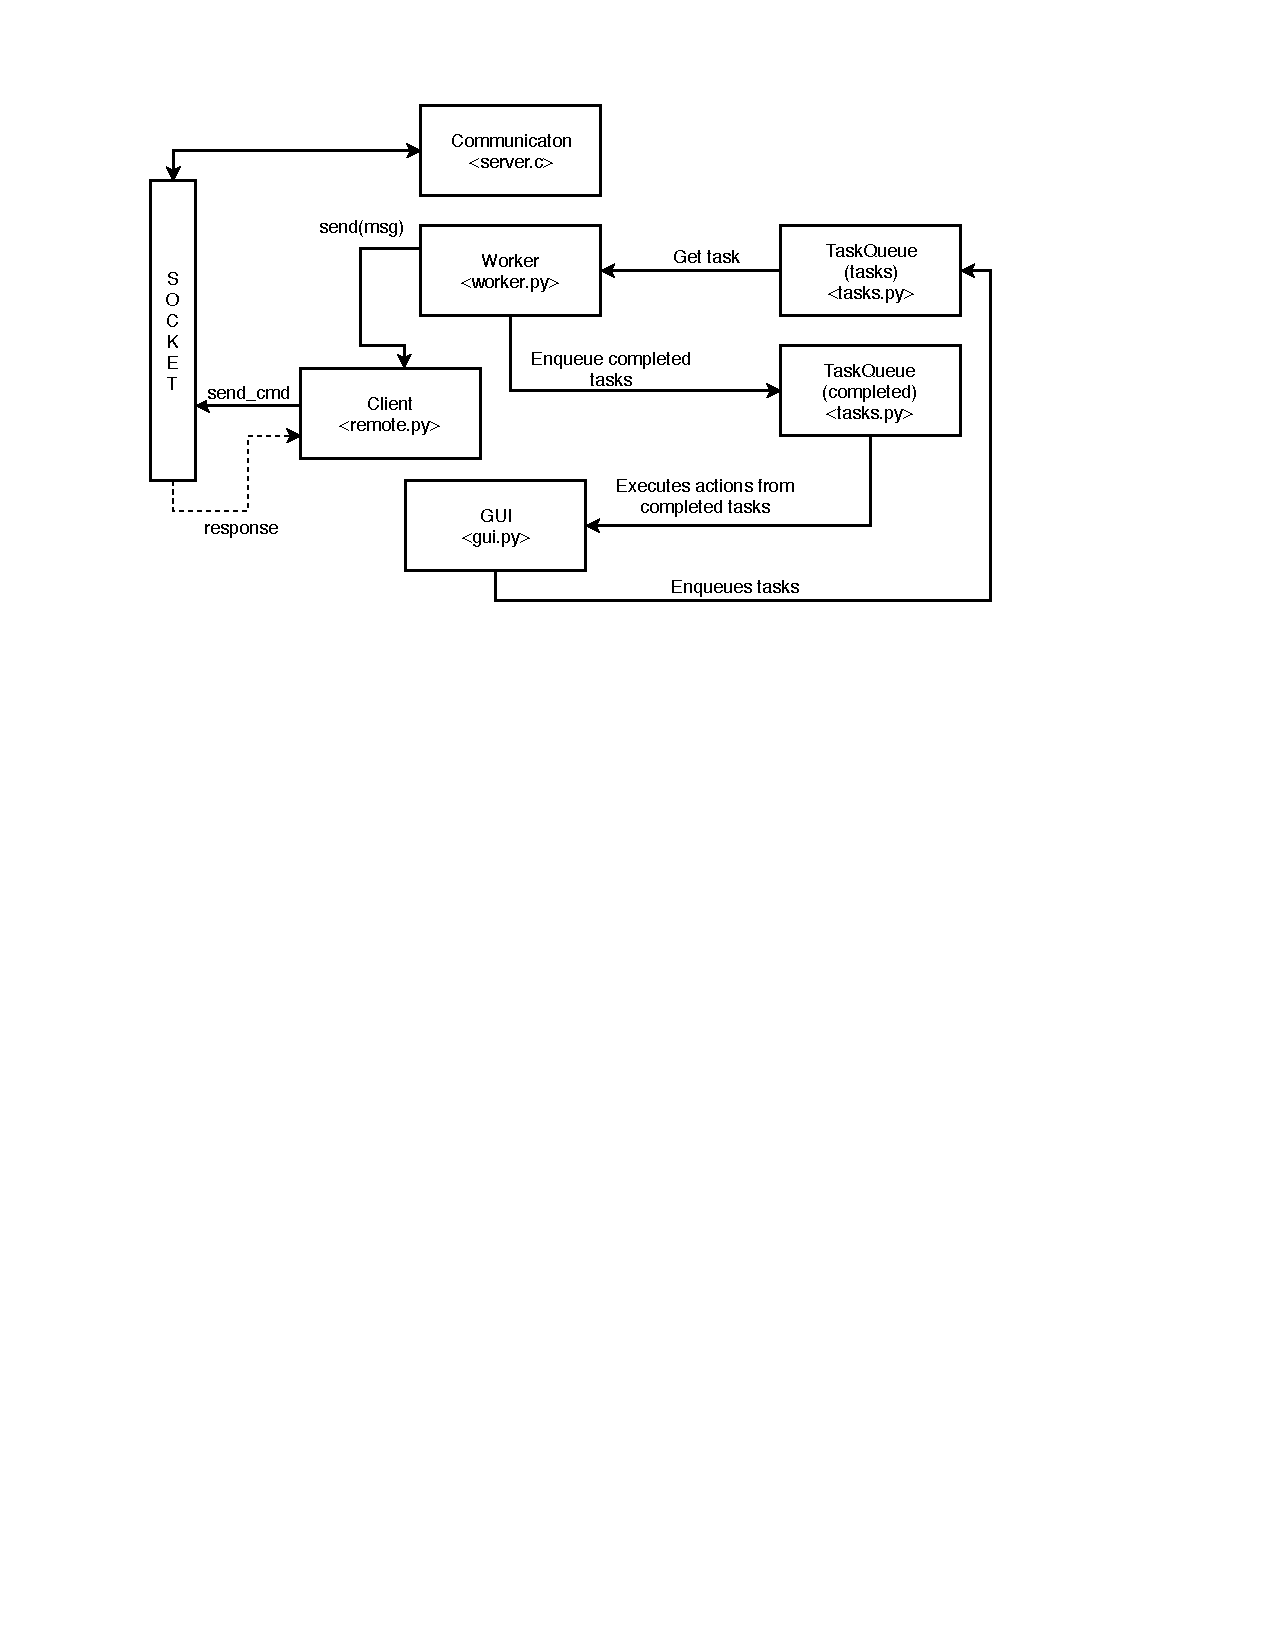
\includegraphics[width=0.6\linewidth]{\figures/client-box-line-diagram.pdf}
	\caption{Ett låd-diagram som beskriver relationen mellan GUI,
	workern och klienten som pratar med servern}
	\label{boxclient}
\end{figure} 

\subsubsection{Trådar}
Programmet skall köras parallellt med två trådar för att förhindra att
gränssnittet fryser för användaren. Programmet kommer behöva vänta på svar från
taxin samt utföra längre beräkningar vilket innebär att programmet kanske inte
hinner uppdatera gränssnittet tillräckligt ofta om det endast använder en tråd.
Synkroniseringen av dessa två trådar sköts av en worker som består av
en stack av tasks och en kö av färdiga 

\subsubsection{Karta och uppdrag}
\label{mission}
Kartan representeras med en riktad graf där varje nod motsvarar en stopplinje
av tejp i vägfältet. Rondeller representeras av infart- och utfartsnoder som
med bågarna bildar en cykel. En båge representerar en enkelriktad körfil från
en stopplinje eller rondell till en annan stopplinje eller rondell. Den här
grafen representeras i sin tur av nedanstående datastrukturer.

% datastrukturer
\begin{labeling}{wwww}
    \item[Karta] Kartan utgörs av en lista med noder.

    \item[Nod] En nod är en klass som består av en nodtyp och en sorterad lista
        av utgående bågar. Det finns tre olika nodtyper; stopplinje,
        parkeringsficka och rondell. 

    \item[Båge] En båge består av ett avstånd och en destination. Den
        representeras av en tuple där första värdet är ett avstånd och det
        andra värdet är en pekare till en nod.
\end{labeling}
Ovanstående datastrukurer är valda för att göra det smidigt att räkna ut den
närmaste vägen med Dijkstras alogritm. Med algoritmen utgår man från en nod och
jämför alla dess grannar. Med ovanstående struktur kan man utgå från startnoden
och därefter
rekursivt gå igenom nodens alla grannar och grannar av grannar. Alternativt,
med en \textit{adjacency list} kräver detta en sökning efter alla bågar som
noden utgår ifrån. Med en \textit{adjacency matrix} måste man kolla igenom
varje element i nodens rad i matrisen och eftersom graferna inte alls är
särskilt täta är det inte särskilt effektiv användning av cykler eller utrymme. 

När en närmaste väg har bestämts ska en kö av kommandon skapas. Detta kan göras
genom att iterera varje nod i vägen och lägga till nedan kommandon för varje
nodtyp. Hur taxin agerar vid varje kommando är specificerat i sektion
\ref{sec:comm-mission}.

\begin{labeling}{wwwwwwwwww}
\item[stopplinje] {\commStop} om markerad som destination, annars \commIgnore.
\item[parkeringsficka] {\commPark} om markerad som destination, annars
\commIgnore 
\item[rondell] En \commEnter, därefter en {\commIgnore} för varje
avfart den ska passera och slutligen en \commExit.
\end{labeling}
För att kunna avgöra vilken avfart taxin ska ta i en rondell är det viktigt att
de utgående bågarna i rondellens nod är sorterade i samma ordning som
avfarterna är placerade i den riktiga banan.

\end{document}
